\section{Results} % 500 words in total
\label{sec:results}

% Overview of numbers


% figure 1 - within class accuracy per model
Within-class accuracy by model can be seen in Figure
\ref{fig:wc_accuracy_x_model} (a sister figure where scores are grouped by
        signature rather than by model can be found in Appendix
\ref{sec:appendixB}).

\begin{figure}
    \centering
    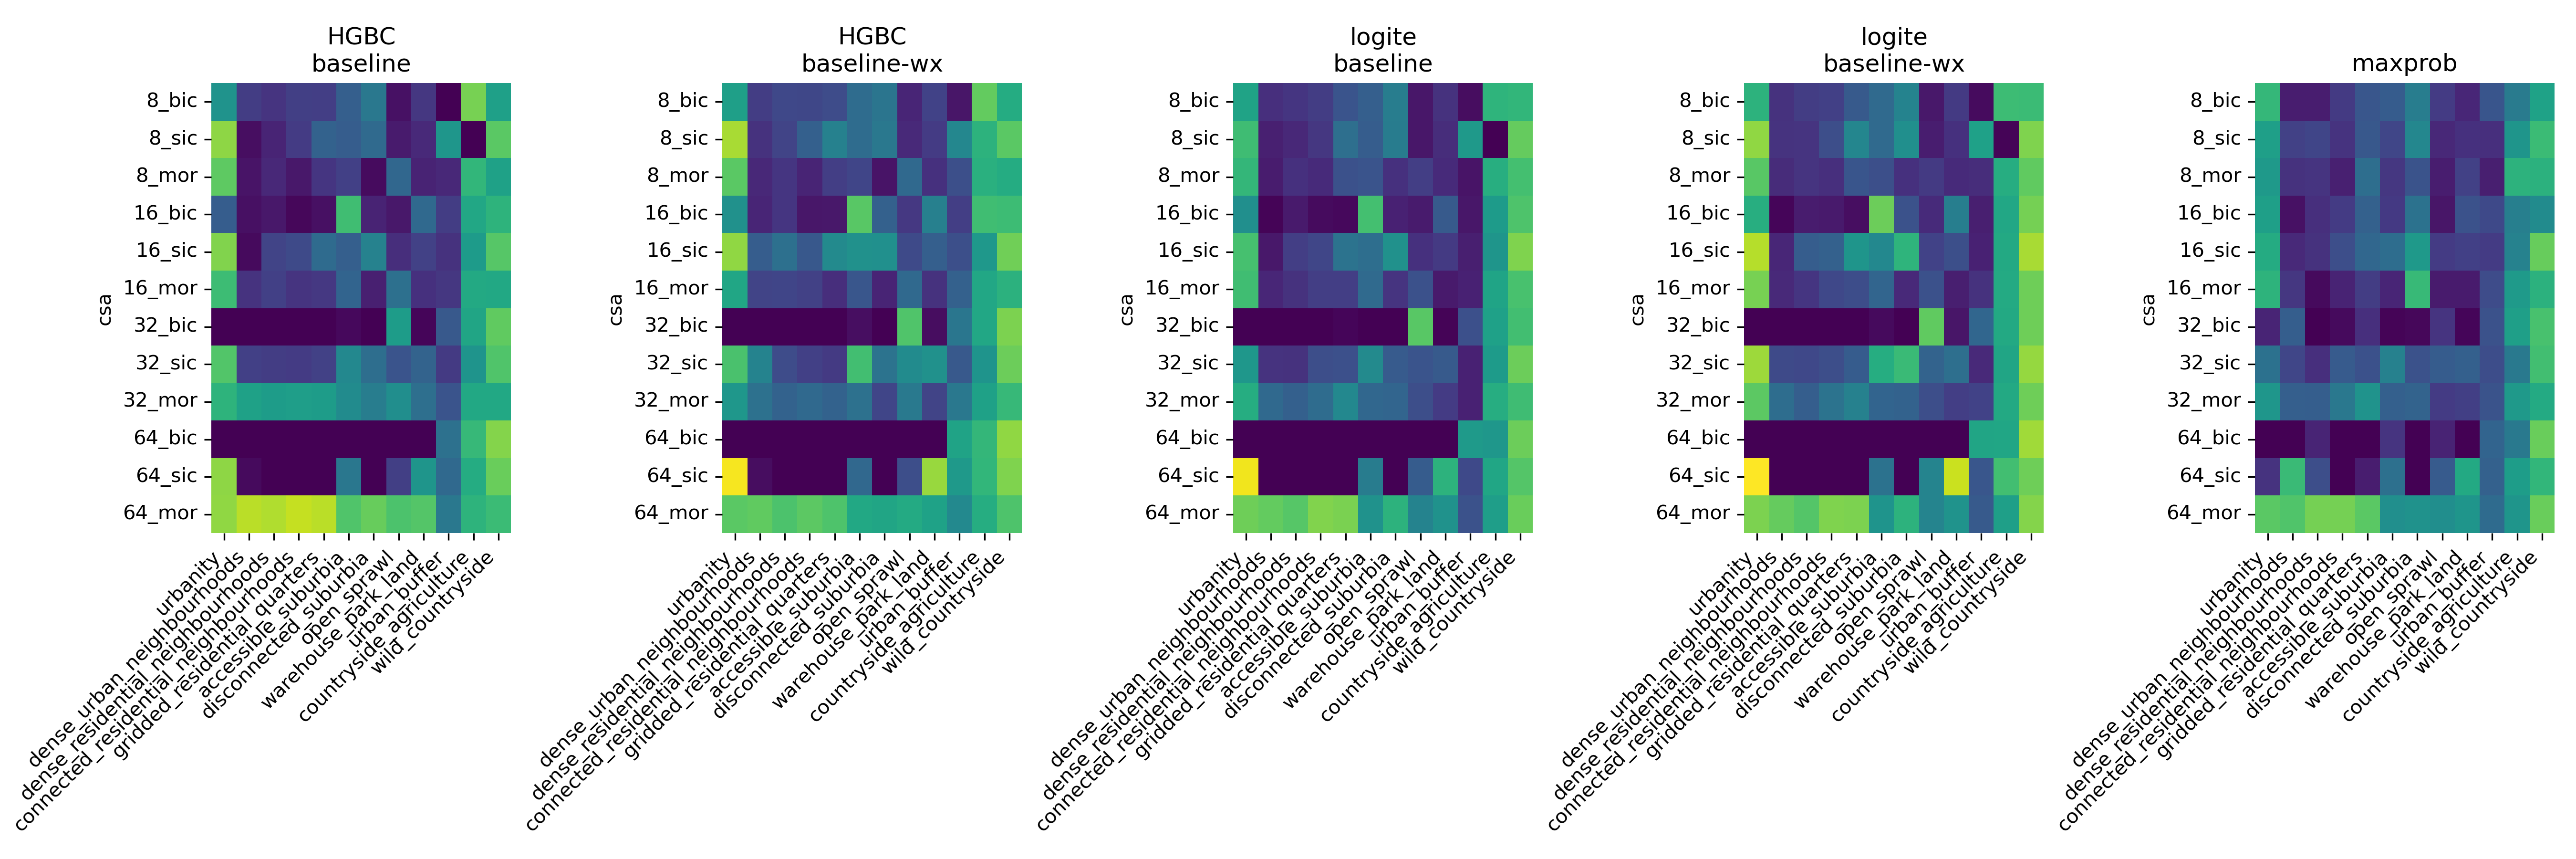
\includegraphics[width=1.0\linewidth]{fig/wc_accuracy_x_model.png}
    \caption{\footnotesize Within-class accuracy scores grouped by model. Each panel
    represents results from one of the five models compared, namely:
    histogram-based boosted classifier (\texttt{HGBC}) with features
    pertaining only to a given chip (\texttt{baseline}) or including also features
    from neighbouring ones (\texttt{baseline-wx}); Logit ensemble
    (\texttt{logite}) with the same two variations; and a simpler maximum
    probability approach (\texttt{maxprob}). Each row in the heatmap
    corresponds to a pair of chipsize (8, 16, 32, and 64 pixels)
    and architechture (baseline image classification, or \texttt{bic}; sliding
            image classification, or \texttt{sic}; and multi-output
    regression, or \texttt{mor}) used in the neural network stage of the
    pipeline. Colouring is standardised across panels and values range from
    0 (dark purple) to 1 (bright yellow).}
    \label{fig:wc_accuracy_x_model}
\end{figure}

Appendix \ref*{sec:appendixC} shows confusion matrices.

% table 1 non spatial, one col for regression
\begin{table}
        \centering
\begin{tabular}{lcccc}
\toprule
{} &    $\kappa$ & Global Accuracy & Macro F1 w. & Macro F1 avg. \\
\midrule
Intercept                                         &  0.2185*** &        0.3236*** &    0.2790*** &      0.1798*** \\
                                                  &   (0.0209) &         (0.0175) &     (0.0174) &       (0.0375) \\
(M) Logit E.                                       &    -0.0245 &         -0.0256* &    -0.0324** &        -0.0325 \\
                                                  &   (0.0168) &         (0.0141) &     (0.0141) &       (0.0302) \\
(M) Max. Prob.                                     &  -0.0559** &       -0.0606*** &    -0.0421** &        -0.0296 \\
                                                  &   (0.0222) &         (0.0187) &     (0.0186) &       (0.0399) \\
(A) M.O.R.                                         &     0.0227 &        -0.0357** &     -0.0278* &      0.1787*** \\
                                                  &   (0.0184) &         (0.0155) &     (0.0154) &       (0.0331) \\
(A) S.I.C.                                         &     0.0232 &          -0.0247 &      -0.0171 &      0.1101*** \\
                                                  &   (0.0184) &         (0.0155) &     (0.0154) &       (0.0331) \\
Chip Size                                         &  0.0036*** &        0.0043*** &    0.0048*** &       0.0014** \\
                                                  &   (0.0004) &         (0.0003) &     (0.0003) &       (0.0006) \\
W                                                 &  0.0572*** &        0.0468*** &    0.0531*** &         0.0392 \\
                                                  &   (0.0168) &         (0.0141) &     (0.0141) &       (0.0302) \\
\midrule
$R^2$                                             &     0.7214 &           0.8281 &       0.8514 &         0.4191 \\
$R^2$ Adj.                                        &     0.6899 &           0.8086 &       0.8346 &         0.3533 \\
N.                                                &     60     &           60     &       60     &         60     \\
\bottomrule
\end{tabular}
    \caption{\label{tab:non_sp_reg}\footnotesize Regression outputs explaining
            global non-spatial
    performance scores. Explanatory variables with a preceding (M) and (A)
    correspond to binary variables for the type of model (with histogram-based
            boosted classifier, or \texttt{HGBC}, as the
    baseline) and architecture (with baseline image classification, or
    \texttt{BIC}, as the baseline),
    respectively. Standard errors in parenthesis. Coefficients significant at
    the 1\%, 5\%, 10\% level are noted with ***, **, and *, respectively.}
\end{table}


\begin{table}
\begin{tabular}{lccc}
\toprule
{}  &       \multicolumn{3}{c}{Within-Class Accuracy} \\
\midrule
Intercept                                         &   0.1866*** &     -0.0237 &    0.0595** \\
                                                  &    (0.0308) &    (0.0311) &    (0.0303) \\
(M) Logit E.                                      &     -0.0125 &     -0.0125 &     -0.0125 \\
                                                  &    (0.0159) &    (0.0141) &    (0.0146) \\
(M) Max. Prob.                                    &     -0.0188 &     -0.0188 &     -0.0188 \\
                                                  &    (0.0211) &    (0.0186) &    (0.0193) \\
(A) M.O.R.                                        &   0.1753*** &   0.2512*** &   0.1753*** \\
                                                  &    (0.0175) &    (0.0163) &    (0.0160) \\
(A) S.I.C.                                        &   0.1202*** &  -0.0783*** &   0.1202*** \\
                                                  &    (0.0175) &    (0.0209) &    (0.0160) \\
Chip Size                                         &   0.0014*** &   0.0041*** &   0.0014*** \\
                                                  &    (0.0003) &    (0.0003) &    (0.0003) \\
1k Obs.                                           &             &   0.0514*** &             \\
                                                  &             &    (0.0036) &             \\
\% Obs.                                           &             &             &   0.0156*** \\
                                                  &             &             &    (0.0013) \\
W                                                 &    0.0365** &   0.0365*** &    0.0365** \\
                                                  &    (0.0159) &    (0.0141) &    (0.0146) \\
(S)Urbanity                                       &   0.2358*** &   0.2022*** &   0.2574*** \\
                                                  &    (0.0349) &    (0.0309) &    (0.0320) \\
(S)Dense urban neighbourhoods                     &  -0.1420*** &  -0.1075*** &  -0.0998*** \\
                                                  &    (0.0349) &    (0.0309) &    (0.0322) \\
(S)Dense residential neighbourhoods               &  -0.1414*** &  -0.0836*** &  -0.0983*** \\
                                                  &    (0.0349) &    (0.0311) &    (0.0322) \\
(S)Connected residential neighbourhoods           &  -0.1306*** &   -0.0726** &   -0.0754** \\
                                                  &    (0.0349) &    (0.0311) &    (0.0323) \\
(S)Gridded residential quarters                   &   -0.0785** &     -0.0127 &     -0.0049 \\
                                                  &    (0.0349) &    (0.0312) &    (0.0326) \\
(S)Disconnected suburbia                          &    -0.0601* &     -0.0103 &     -0.0019 \\
                                                  &    (0.0349) &    (0.0311) &    (0.0324) \\
(S)Open sprawl                                    &   -0.0845** &  -0.0995*** &  -0.1143*** \\
                                                  &    (0.0349) &    (0.0309) &    (0.0321) \\
(S)Warehouse park land                            &   -0.0857** &   -0.0788** &   -0.0817** \\
                                                  &    (0.0349) &    (0.0309) &    (0.0320) \\
(S)Urban buffer                                   &   -0.0828** &  -0.1382*** &  -0.1753*** \\
                                                  &    (0.0349) &    (0.0311) &    (0.0330) \\
(S)Countryside agriculture                        &   0.2236*** &   0.1593*** &   0.1118*** \\
                                                  &    (0.0349) &    (0.0312) &    (0.0334) \\
(S)Wild countryside                               &   0.3876*** &   0.3283*** &   0.2925*** \\
                                                  &    (0.0349) &    (0.0311) &    (0.0330) \\
\midrule
$R^2$                                             &      0.4979 &      0.6087 &      0.5794 \\
$R^2$ Adj.                                        &      0.4857 &      0.5987 &      0.5686 \\
N.                                                &      720    &      720    &      720    \\
\bottomrule
\end{tabular}
    \caption{\label{tab:non_sp_reg_wc}\footnotesize Regression outputs explaining
            within-class accuracy. Explanatory variables with a preceding (M),
            (A) and (S)
    correspond to binary variables for the type of model (with histogram-based
            boosted classifier, or \texttt{HGBC}, as the
    baseline), architecture (with baseline image classification, or
    \texttt{BIC}, as the baseline) and spatial signature (with Accessible
    suburbia as the baseline),
    respectively. Standard errors in parenthesis. Coefficients significant at
    the 1\%, 5\%, 10\% level are noted with ***, **, and *, respectively.}
\end{table}

% figure 2 - map for a single class target/prediction/

\begin{figure}
    \centering
    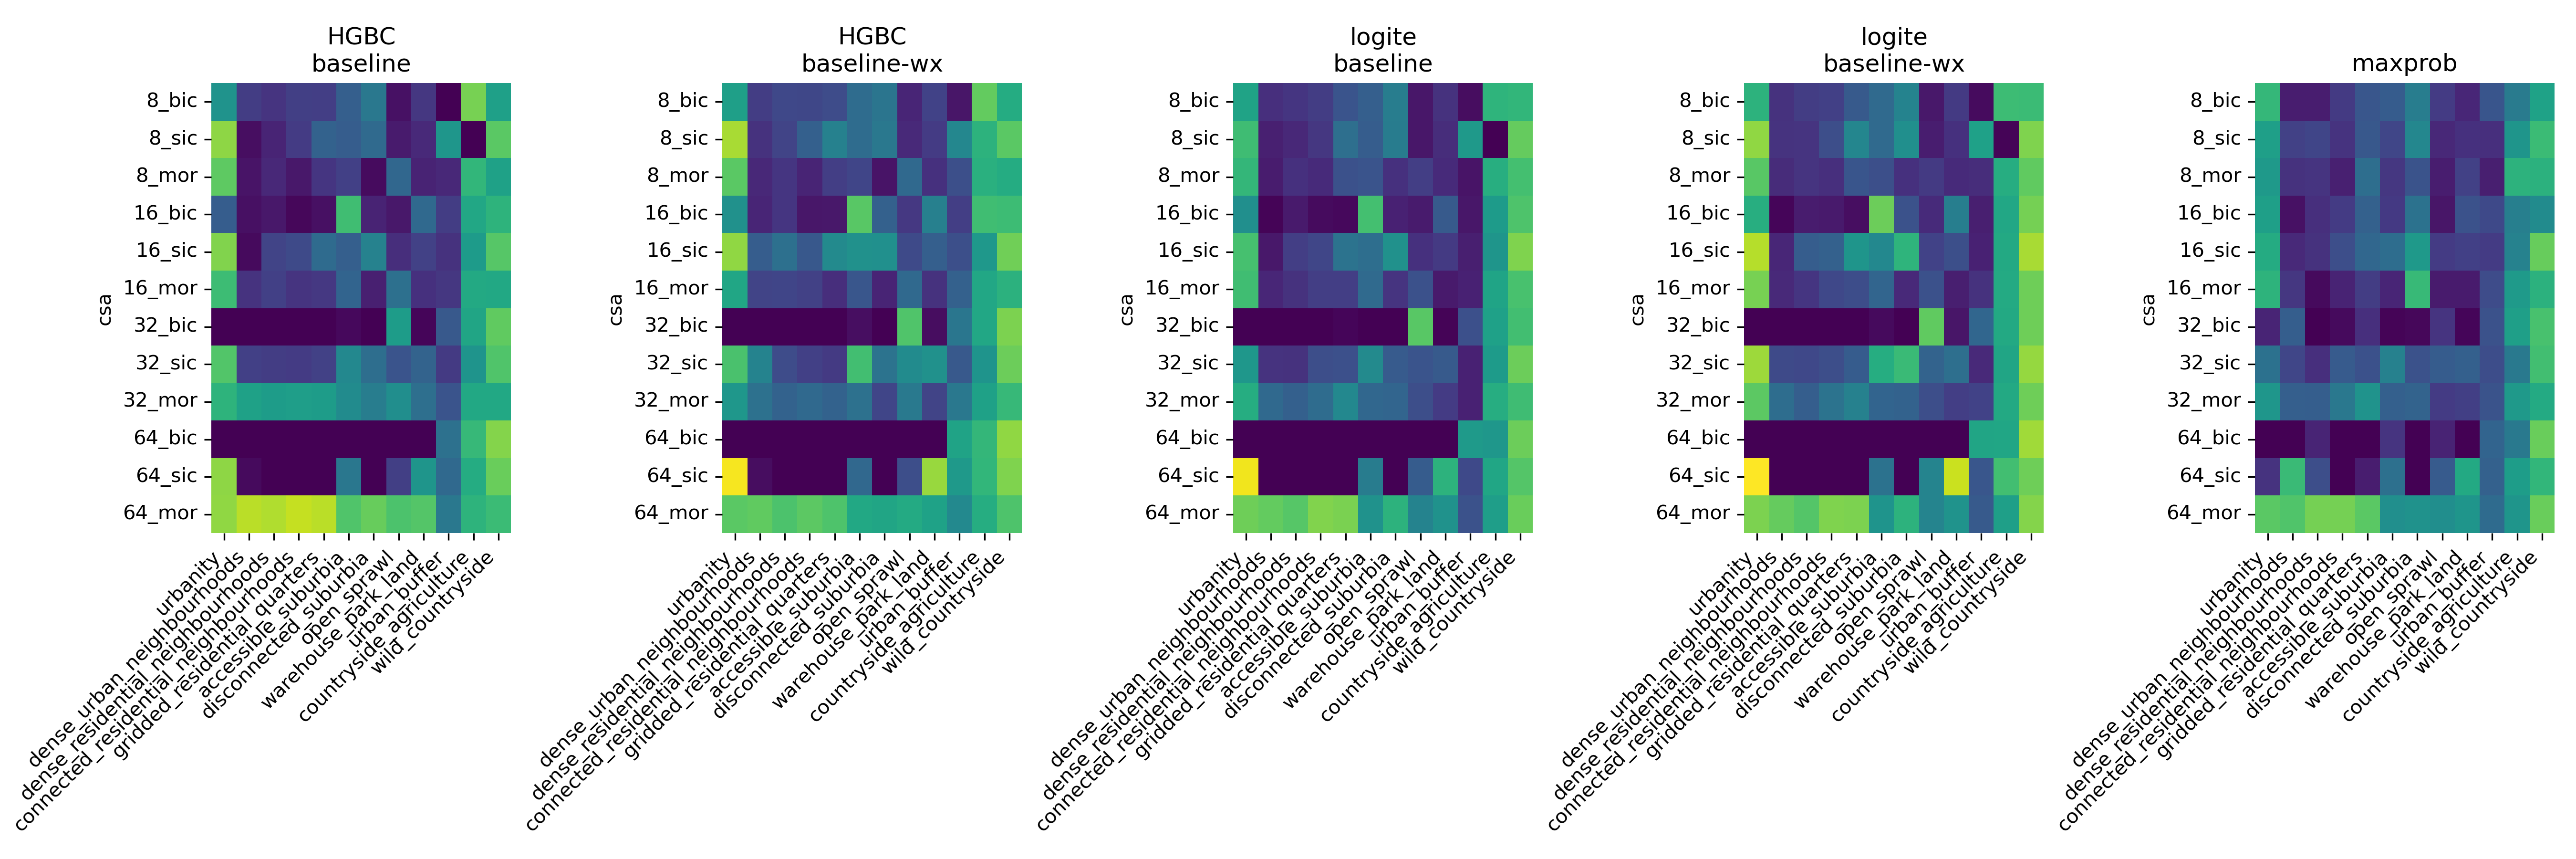
\includegraphics[width=1.0\linewidth]{fig/wc_accuracy_x_model.png}
    \caption{\footnotesize TBC}
    \label{fig:prediction_comparison_maps}
\end{figure}


% table 2 spatial,



